% !TEX encoding = UTF-8 Unicode
\documentclass[a4paper]{article}

\usepackage[utf8]{inputenc}
\usepackage[T1]{fontenc}
\usepackage{amsmath}
\usepackage{amsfonts}
\usepackage{graphicx}

\author{A.U. Thor} %Declaring the author for the maketitle command
\title{A primer on \LaTeX} %Declaring the title for the maketitle command
\date{\today} %Declaring the date for the maketitle command. \today prints the current date. You can write anything, including things that are not a date. 

\begin{document}

\maketitle

\tableofcontents

\section{Introduction}

We are going to construct now a template or sample document which covers the main tools that one needs to produce a complex \LaTeX{} document. Most of the things that you will ever need and many more are covered throughly in \cite{MittelbachGoossens2004}. In the next lecture we are also going to cover some more advanced material to understand how the internals of \LaTeX{} work. This is rarely used directly but it helps to understand why \LaTeX{} does things the way it does and it saves time. All the details can be found in the book by the father of \TeX, D. Knuth \cite{Knuth1990}.

\section{The Preamble}

About the encodings and how to use them. I can type é í ó without trouble.

\section{Title and other headings}

This formatting depends on the class, as many others. Typically the style and macros used to define the headings of the document depend on the journal or editorial where you will publish the document. The article class (as well as book and report) include a simple way of producing this heading. There are some macros like \textbackslash{}author, \textbackslash{}title, \textbackslash{}date which then are transformed using the \textbackslash{}maketitle command. In the article class the \textbackslash{}maketitle needs to be included after the \textbackslash{}begin\{document\} statement. The rest of the macros will go typically in the preamble. Check how they are used in the source file.


\section{Table of contents}

%\tableofcontents

\section{Mathematics in a Document}

\subsection{The math modes and the text mode}

Typesetting mathematics in a document was one of the reasons why \TeX{} and later \LaTeX{} was created. There are two types of math modes inline mode and displayed mode. Inline mode is when an equation or mathematical expression is embedded in the text, $\sum_{j=1}^{n=10}x^j$, like this one. It is included in the source text with the symbol \$. A single \$ starts the inline math mode and another \$ ends it. Another way of inserting math in the inline mode is surrounding it with the symbols \textbackslash(, \textbackslash), like here  \(\lim_{x\to\infty} f(x) = 7\). The math mode and the text mode have many differences. For instantes, regular latin characters are displayed in italics and spaces are ignored $This is math mode$. Display mode can be called using double dollar symbols \$\$,\$\$ or enclosing it with \textbackslash[, \textbackslash] like here $$\sum_{j=1}^{n=10}x^j$$ or \[\lim_{x\to\infty} f(x) = 7.\]

As opposed to inline math mode, the displayed mode prints the mathematical expression in a separated line. Wether this equation is centered, right aligned or left aligned depends on the class and styling. Notice that there are differences in how the math is typeset in the two modes. The inline mode is more compact and sub and superscripts are placed at different positions.

\subsection{Some environments useful for presenting equations}

  \begin{equation}\label{my_equation}
    \int_{\infty}^\infty e^{-x^2} dx = \sqrt{\pi}
  \end{equation}

I can point to the equation \ref{my_equation}. 

% The following requires amsmath. Speak abou packages and funcvtionalities.

  \begin{align}
    (a+b)^2 &= a^2 + 2ab + b^2 \\
      & \geq 0 \\
      & > - x^2 +5 \notag
   \end{align}

  \begin{align*}
    (a+b)^2 &= a^2 + 2ab + b^2 \\
      & \geq 0 \\
      & > - x^2 +5
  \end{align*}
   
\subsection{Tabular math}

  %matrix, pmatrix, bmatrix, cases

  $$%
    A = %
    \begin{bmatrix}
      a & b \\ c & d
    \end{bmatrix}
  $$


  $$
  f(x ) = %
    \begin{cases}
      \exp\left(-\frac{1}{x}\right) &, \text{if } x > 0 \\
      0 &, \text{if } x\leq 0
    \end{cases}
  $$


\section{Tables in text mode. The tabular environment}

One can produce tables in latex. We will speak about the basic functionality. The functionality can be extended by using packages that can be loaded in the preamble. 

\begin{tabular}{l c r | c} % Warning, small L is l and the pipe |. They are typeset very similar. Small L is for left alignment will the pipe is to include a vertical line between the columns.
Aligned lef & An Oak &  Aligned right & An Oak \\
$\emptyset$ & Centered & $\emptyset$ &  Centered \\
\hline %This command puts a horizontal line in the table
$\emptyset$ & $\emptyset$ & $\emptyset$ &  $\emptyset$ \\
\end{tabular}


\section{List environments}

\begin{itemize}
  \item First element
  \item Second element
\end{itemize}

\begin{enumerate}
  \item First element
  \item Second element
\end{enumerate}

\begin{enumerate}
  \item First element
    \begin{enumerate}
      \item element 1.1
      \begin{enumerate}
        \item element 1.1.1
        \item element 1.1.2
        \item element 1.1.3
      \end{enumerate}
      \item element 1.2
    \end{enumerate}
  \item Second element
\end{enumerate}

The labels of the nested enumerate environment can be changed. This is done with the special commands 
%\labelenumi, \labelenumii \labelenumiii
%\theenumi %\theenumii

\theenumii 

\theenumiii

\renewcommand\theenumii{\Roman{enumii}}

\theenumii

\begin{enumerate}
  \item First element
    \begin{enumerate}
      \item element 1.1
      \begin{enumerate}
        \item element 1.1.1
        \item element 1.1.2
        \item element 1.1.3
      \end{enumerate}
      \item element 1.2
    \end{enumerate}
  \item Second element
\end{enumerate}


\renewcommand\labelenumii{\theenumii]] ->}

\begin{enumerate}
  \item First element
    \begin{enumerate}
      \item element 1.1
      \begin{enumerate}
        \item element 1.1.1
        \item element 1.1.2
        \item element 1.1.3
      \end{enumerate}
      \item element 1.2
    \end{enumerate}
  \item Second element
\end{enumerate}

We will see more functionality of the command \textbackslash{}renewcommand. This is very useful and a must-to-know for every \LaTeX user.

\section{Changing Fonts in a \LaTeX Document}

\begin{itemize}

\item Series 

  \begin{itemize}
    \item Bold; \textbf{I am Bold}; {\bfseries I am bold}

    \item Medium(default); \textmd{ I am normal}; {\mdseries I am normal} ; {\mdseries I am normal}

      \textbf{ This is bold \textmd{this is not} } 
  
  \end{itemize}

\item Family

  \begin{itemize} 
    \item Serif font (default); \textrm{Here am I }; {\rmfamily Here am I};

    \item Sans Serif font; \textsf{Here am I}; {\sffamily Here am I}
    
    \item Typewriter font; \texttt{text}; {\ttfamily Here am I }

  \end{itemize}

\item Shape

  \begin{itemize}
    \item upright (default); \textup{Normal}; {\upshape also normal}
    \item slanted/italics; \textit{I am in italics}; {\itshape Also in italics}
    \item small caps: \textsc{I am In Small Caps}; {\scshape i am Also}
  \end{itemize}

\end{itemize}

You can mix the three properties, some particular combinations might not be available: {Hello} {\ttfamily \itshape Hello} {\sffamily \itshape Hello} {\sffamily \bfseries Hello} {\bfseries Hello} {\ttfamily \bfseries Hello} {}

\section{Defining macros}

%\newcommand\newcommandname{code to be substituted when \newcommandname is written}
%\renewcommand...

\newcommand\R{\mathbb{R}} %\mathbb requires the amsfonts package


$\R$

Commands with arguments

\newcommand\average[1]{\langle#1\rangle}

$\average{A}$

\newcommand\fraction[2]{\frac{#1}{#2}}

$\fraction{\text{Numerator}}{\text{Denominator}}$


\section{Including Graphics}

\begin{figure}[h]
  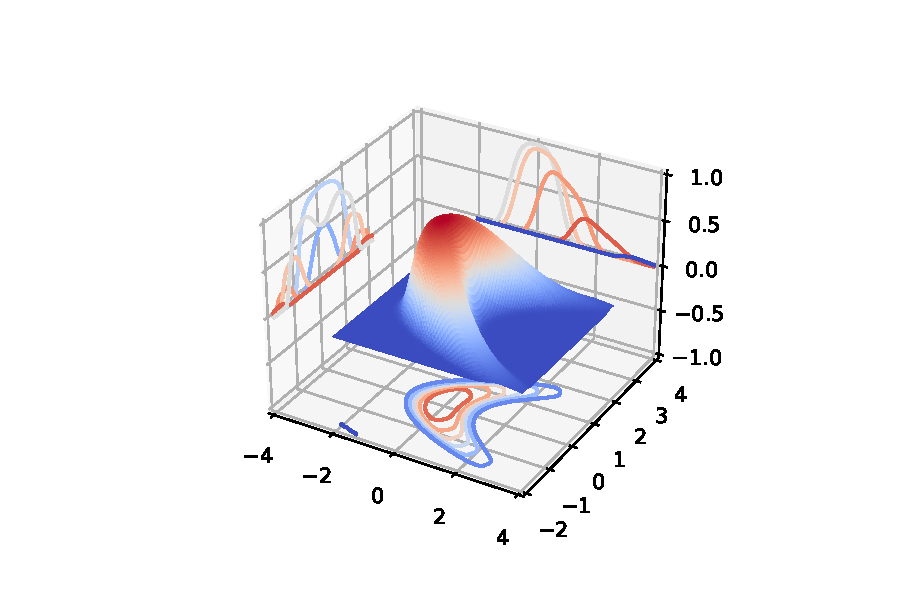
\includegraphics{3dplot.pdf}
  \caption{Some descriptive text}\label{referencefigure}
\end{figure}





\section{Defining a bibliography with `Bibtex'}

We have referenced the bibliography previously, like here \cite{Stone1932}. With \LaTeX{} one can use an automated tool to generate the bibliography, this is called `Bibtex'.  For doing it one needs to include the two statements that can be found after this paragraph. The source document needs to be parsed several times to complete the process. This is so because first one needs to know which references in the `.bib' file are cited in the document. Then a formatted bibliography file `.bbl' is created. Then the bibliography file is read and included in the document. Finally you need to run latex again to get the references properly. In summary, whenever you add some \textbackslash{}cite references to the document you need to compile with latex, then `Bibtex' and then with \LaTeX{} two times again. 

% Different bibliography styles. plain, siam, abbrv, alpha

\bibliographystyle{siam}
\bibliography{my_bibliography.bib}














\end{document}














